\section{Introduction}
Molecular docking predicts a bound conformation of a ligand in a protein binding site and is used to prioritise
compounds and to form binding-mode hypotheses \citep{trott2010vina,eberhardt2021vina,pagadala2017review}.
Learned post-docking correction is an attractive complement: a model that sees the docked ligand and its pocket
can predict a residual displacement towards the experimentally observed pose. The risk is asymmetric. A
correction can rescue a poor pose, but the same operation can move an acceptable pose out of tolerance, and it can
do so while producing a molecule whose bond lengths, angles or contacts are physically implausible---a failure that
root-mean-square deviation (RMSD) cannot see \citep{buttenschoen2024posebusters}.

\citet{mwamughunda2026original} studied this risk with a confidence-gated correction model: a ligand--pocket
cross-attention network with a coordinate-correction head and a heteroscedastic log-variance head, a confidence
gate calibrated on validation data only, and an evaluation on three axes (continuous error, RMSD-threshold
transitions, and a PoseBusters chemical-validity audit). Their central findings were that ungated correction
reduces mean squared error while lowering or leaving unchanged RMSD-threshold success, that it collapses chemical
validity, and that gating recovers validity only partially, less so on an externally shifted cohort.

These conclusions matter beyond one model, because they concern how learned refinement should be evaluated. They
also rest on one dataset construction, one split, and a gate whose threshold is an absolute uncertainty value. This
paper therefore asks two questions. \textbf{(Q1) Reproducibility:} do the original findings hold when the full
pipeline is rebuilt independently from public sources, using the same datasets and protocol? \textbf{(Q2) Gaps:}
can the failure modes the original study diagnosed---validity loss, miscalibration under shift, and single-split
evidence---be measured more precisely or mitigated with label-free changes to the decision rule?

Our contributions are:
\begin{enumerate}
\item An independent, end-to-end reconstruction of the study from public data: the PDBbind\,v2020 P-L, LP-PDBBind
      and MISATO identifier intersection, an external PoseBusters cohort, AutoDock Vina docking, four candidate pocket
      encoders, the three-stage gate, and a full-cohort PoseBusters audit, with every deviation reported (Section~\ref{sec:deviations}).
\item A side-by-side comparison of every headline number of the original study with the reproduction (Table~\ref{tab:compare}).
\item Seven new analyses addressing gaps identified in the original work (G1--G7): a quantile-matched gate that
      adapts to uncertainty shift without labels, a validity-veto gate, rigid-body projection of the correction, deep-ensemble
      uncertainty, sequence-level leakage between the training and external cohorts, a diagnosis of the uncertainty
      shift, and split-to-split variance over three alternative splits.
\item A public code release that regenerates every number and figure in this paper.
\end{enumerate}

\section{Related work}
Classical docking balances conformational search and scoring \citep{meng1992dock,morris2009autodock4,trott2010vina};
AutoDock Vina\,1.2 added a Python interface used here \citep{eberhardt2021vina}. PDBbind is the standard source of
characterised complexes \citep{wang2004pdbbind,wang2005pdbbind_update}; LP-PDBBind reorganises it to reduce
train--test leakage \citep{li2023lppdbbind}, and MISATO adds molecular-dynamics trajectories for most PDBbind
complexes \citep{siebenmorgen2024misato}. Learned docking methods predict poses directly or generatively
\citep{stark2022equibind,corso2023diffdock,pei2023fabind}, and general structure predictors now model complexes
\citep{jumper2021alphafold,abramson2024af3}. PoseBusters showed that many learned methods produce poses that pass RMSD
criteria but fail basic physical checks, and that performance drops on proteins dissimilar to the training data
\citep{buttenschoen2024posebusters}. Later benchmarks report similar gaps between geometric accuracy and physical or
interaction validity \citep{morehead2026posebench,errington2025interaction,li2025limits,gu2025vs}.

Heteroscedastic regression models input-dependent noise through a learned variance \citep{kendall2017uncertainty}; deep
ensembles estimate uncertainty from model disagreement \citep{lakshminarayanan2017ensembles}; calibration methods map
scores to reliable probabilities \citep{guo2017calibration,kuleshov2018calibrated}. Uncertainty estimates degrade under
dataset shift \citep{ovadia2019shift,quinonero2009shift}, including for protein--ligand affinity \citep{rayka2025uq}.
Our quantile-matched gate borrows the rank-based view of conformal prediction \citep{vovk2005alrw}: it fixes the
fraction of cases admitted rather than an absolute score.

\section{Materials and methods}
The pipeline (Fig.~\ref{fig:method}) follows the original protocol stage by stage. All stages are deterministic given
the released manifest and fixed seeds.

\begin{figure}[H]
\centering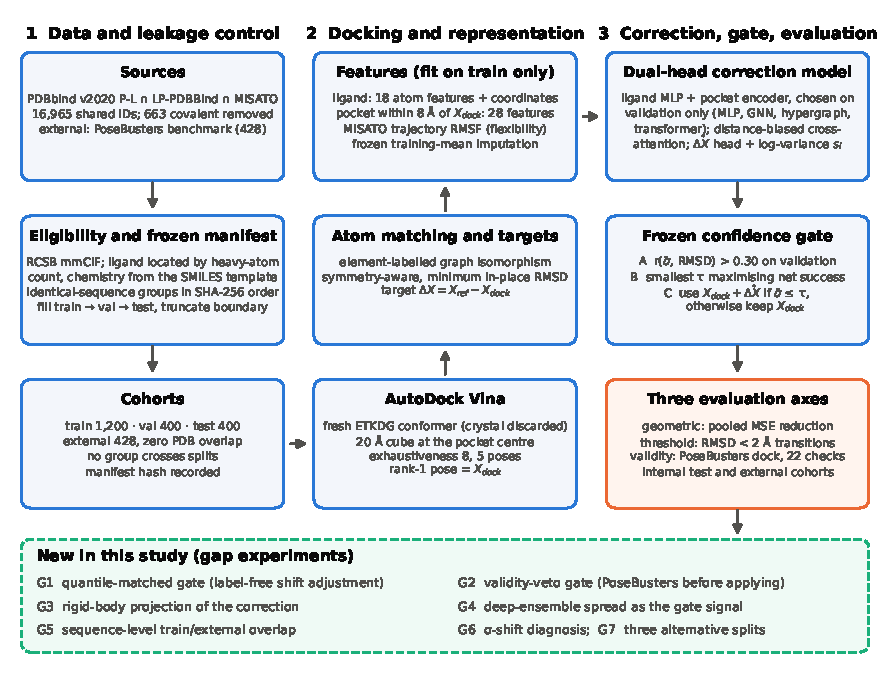
\includegraphics[width=\linewidth]{fig01_methodology.pdf}
\caption{Methodology. Column 1 builds the leakage-controlled cohorts, column 2 docks each complex and builds its
representation, column 3 trains the dual-head correction model, applies the frozen confidence gate and evaluates every
pose on three axes. The band lists the new analyses G1--G7 (G8, the deformation analysis, is in Section~\ref{sec:results}).}
\label{fig:method}
\end{figure}

\subsection{Datasets and eligibility}
\paragraph{Internal pool.} The PDBbind\,v2020 P-L set (19{,}443 complexes, as distributed in LP-PDBBind) was intersected
with the MISATO MD identifier lists (train, validation and test files; 16{,}972 identifiers), giving \IntersectN{} shared
complexes (original study: 16{,}627). \CovalentN{} covalent complexes were excluded using the LP-PDBBind flag. Structures
were downloaded from the RCSB PDB \citep{berman2000pdb} as mmCIF. The crystal ligand was located as the single
non-polymer residue whose heavy-atom count equals that of the LP-PDBBind SMILES and whose coordinates admit the SMILES
bond orders (RDKit \texttt{AssignBondOrdersFromTemplate}); the ligand was then sanitised with RDKit. Ligands spanning
several residues (mostly peptides) cannot be located this way and were excluded (\LigNotLocated{} complexes), as were
\StructFail{} entries whose structures failed to parse. The receptor retains polymer residues, metal ions and organic
cofactors, and drops water, common crystallisation additives, hydrogens, the ligand, and any hetero group within
1\,\AA{} of a ligand atom (alternate ligand copies).

\paragraph{External cohort.} The 428-complex PoseBusters benchmark set \citep{buttenschoen2024posebusters}, with its
supplied receptor and ligand files. Internal--external PDB-identifier overlap is zero.

\paragraph{Leakage-controlled manifest.} Complexes were grouped by identical protein sequence (LP-PDBBind chain
sequence). Groups were ordered by the SHA-256 digest of the group identifier and used to fill the training (1{,}200),
validation (400) and internal-test (400) splits in that order; only the boundary group is truncated and its unselected
members retired. Eligibility was checked before a complex took a slot. The manifest (SHA-256 recorded) was frozen before
any modelling. No group crosses splits.

\subsection{Docking and atom matching}
For each complex a fresh conformer was generated from the ligand graph with ETKDG and MMFF94 optimisation
\citep{riniker2015etkdg,halgren1996mmff}, discarding the crystal coordinates, and prepared with Meeko. Receptors were
converted to PDBQT with Open Babel \citep{oboyle2011openbabel}; receptor atoms of types Vina cannot score were removed.
AutoDock Vina was run with a 20\,\AA{} cubic box at the crystal-ligand centroid (pocket-informed), exhaustiveness 8, five
poses and a fixed seed; the rank-1 pose is the baseline $X_{dock}$. Docked and reference heavy atoms were matched by
element-labelled graph isomorphism, choosing among graph automorphisms the correspondence with the smallest in-place
RMSD (symmetry-corrected RMSD, no superposition). Complexes whose graphs did not match were excluded.

\subsection{Pocket representation and MISATO flexibility}
The pocket is the set of residues with any heavy atom within 8\,\AA{} of a docked ligand heavy atom, so it is defined
from the docked pose alone. Each residue node has 28 features: a 20-way amino-acid one-hot encoding, the C$\alpha$
position and side-chain-centroid offset relative to the docked-ligand centroid, a local degree (C$\alpha$ neighbours
within 10\,\AA{}), and a flexibility value. Ligand atoms carry 18 chemistry features (element, degree, aromaticity,
ring membership, formal charge, hydrogen count, hybridisation) and their coordinates. Edges link C$\alpha$ pairs
within 10\,\AA{}; hyperedges are chain segments of consecutive residues.

Flexibility is the per-residue root-mean-square fluctuation (RMSF) of the MISATO trajectory. Because the 133\,GB MISATO
file could not be stored, each complex's trajectory (100 frames) was read remotely by HTTP range requests. MISATO
coordinates are expressed in a different frame and residue numbering, so frame~0 was registered onto the crystal by
matching the ligand's heavy-atom graph (element-labelled isomorphism) and a Kabsch fit \citep{kabsch1976}; frames were
aligned on protein heavy atoms before computing per-atom RMSF, and each pocket residue receives the mean RMSF of MISATO
atoms within 1.5\,\AA{} of its heavy atoms. Registrations with ligand RMSD above 2\,\AA{} or median protein
nearest-neighbour distance above 2.5\,\AA{} were rejected. Residues without a mapped atom, complexes with rejected
registrations, and all external complexes receive the frozen training-set mean, the original study's prespecified
imputation rule. Continuous features and the coordinate scale were fitted on training complexes only.

\subsection{Correction model and uncertainty}
For $N$ matched atoms the target is $\Delta X = X_{ref} - X_{dock}$, the model predicts
$\hat{\Delta X} = f_\theta(X_{dock}, G_{pocket})$, and the corrected pose is $X_{corr} = X_{dock} + \hat{\Delta X}$.
The common architecture has a ligand MLP encoder, a pocket encoder, distance-biased cross-attention from ligand atoms to
pocket residues, a three-coordinate correction head and a per-atom log-variance head $s_i$ (clamped to $[-12,12]$), with
$\sigma_i = \exp(s_i/2)$. The training objective is the heteroscedastic negative log-likelihood
\begin{equation}
\mathcal{L}_{NLL} = \tfrac{1}{2}\,\mathrm{mean}_i\!\left[3 s_i + \lVert \hat{\Delta X}_i - \Delta X_i \rVert_2^2 / e^{s_i}\right].
\end{equation}
The four candidate pocket encoders are an MLP over residue features, a distance-weighted message-passing GNN
\citep{gilmer2017mpnn}, a residue-incidence hypergraph encoder with flexibility-weighted segment attention, and a
transformer with a learned distance bias. All use hidden size 64 and two encoder layers, and are trained with Adam
(learning rate $10^{-3}$), at most 15 epochs and patience 5 on validation NLL, with random proper rotations of all
coordinates and targets during training only. Five seeds (0, 42, 123, 999, 2026) were trained per architecture; the
architecture with the highest mean validation pooled MSE reduction was selected. Held-out data were not used for
selection.

\subsection{Confidence gate}
Let $\bar\sigma_j$ be the mean predicted $\sigma$ of seed--complex row $j$. Stage~A requires the pooled validation Pearson
correlation between $\bar\sigma$ and baseline RMSD to exceed 0.30. Stage~B sweeps every distinct validation $\bar\sigma$
and selects the smallest threshold maximising pooled validation net success,
\begin{equation}
\tau = \min\{t : \mathrm{NetSuccess}(t) = \max_{t'} \mathrm{NetSuccess}(t')\},
\end{equation}
where NetSuccess is the RMSD\,$<$\,2\,\AA{} success rate when the correction is applied to rows with $\bar\sigma_j \le t$
minus the baseline success rate. Stage~C applies the frozen $\tau$ to held-out data without adjustment.

\subsection{Evaluation}
\emph{Geometric:} pooled MSE reduction $100\,(\mathrm{MSD}_{base}-\mathrm{MSD}_{corr})/\mathrm{MSD}_{base}$ over all atoms.
\emph{Threshold:} success is RMSD\,$<$\,2\,\AA{}; transitions are preservation (success$\to$success), harm (success$\to$failure),
rescue (failure$\to$success) and persistent failure. \emph{Validity:} the full PoseBusters \texttt{dock} configuration
(22 binary checks: loading, sanitisation, InChI, connectivity, radicals, bond lengths and angles, internal clash, ring
and double-bond flatness, internal energy, and protein-ligand distance and volume-overlap checks), applied to heavy-atom
poses against the receptor; a pose is valid only if every check passes, and a check not computed after an upstream
failure counts as failed. Gated poses are the corrected pose when the gate fires, otherwise the baseline. Uncertainty
intervals are reported in two ways: a Student-$t$ interval over the five seed-level rates, and a 10{,}000-resample paired
complex-level percentile bootstrap.

\paragraph{Statistical validation.} A training-only permutation test relates each atom's distance to the nearest pocket
C$\alpha$ to its target displacement magnitude, shuffling magnitudes within complexes (10{,}000 permutations). A rotational
audit compares predictions before and after a random rotation (rotated back) for ten validation complexes and five seeds.
A synthetic identity check verifies $\mathrm{RMSE}_{component} = \mathrm{RMSD}/\sqrt{3}$.

\subsection{New analyses (G1--G7)}\label{sec:gaps}
\begin{description}
\item[G1 Quantile-matched gate.] The validation admit fraction $q$ is frozen; each held-out cohort is gated at the
      $q$-quantile of its own $\bar\sigma$ distribution. No held-out label is used. This tests whether matching the admit
      rate, rather than the absolute threshold, removes the effect of uncertainty-scale shift.
\item[G2 Validity veto.] A correction is applied only if the corrected pose passes all PoseBusters checks (alone, and
      combined with the $\sigma$ gate). PoseBusters needs only the pose and receptor, so the rule is deployable.
\item[G3 Rigid-body projection.] The free per-atom correction is replaced by the rigid motion of the docked pose that
      best fits it (Kabsch). Internal geometry is preserved by construction; the gate is recalibrated on validation with
      the same rule.
\item[G4 Deep-ensemble uncertainty.] The five seeds' mean correction is gated by their spread (mean per-atom standard
      deviation), calibrated exactly as in Stage~B; a rigid-projected variant is also evaluated.
\item[G5 Sequence-level leakage.] Exact and near-identical (3-mer Jaccard $\ge$ 0.9) chain-sequence overlap between the
      training set and the external cohort, and outcomes stratified by overlap.
\item[G6 Uncertainty-shift diagnosis.] Per-cohort $\bar\sigma$ distributions (two-sample Kolmogorov--Smirnov tests),
      $\sigma$--RMSD correlation per cohort, and cohort descriptors (ligand size, pocket size).
\item[G7 Split variance.] The docked internal pool is re-partitioned three times with the same group-aware rule and
      different hash salts; the selected architecture is retrained (five seeds each) and re-evaluated.
\end{description}

\subsection{Deviations from the original protocol}\label{sec:deviations}
\begin{itemize}
\item \emph{Structures:} PDBbind's curated files require registration, so structures came from the RCSB PDB and ligand
      chemistry from LP-PDBBind SMILES. Multi-residue ligands were excluded (the original study excluded none for this
      reason).
\item \emph{Grouping:} identical protein sequence was used as the leakage group; the original used LP-PDBBind grouping
      (1{,}792 candidate-touching groups versus \TouchedGroups{} here).
\item \emph{Software:} AutoDock Vina 1.2.7 (original: 1.2.0), RDKit 2026.09, PoseBusters 0.6.5.
\item \emph{Docked-pose export:} Meeko's RDKit export was used instead of an Open Babel PDBQT$\to$SDF conversion; the
      Open Babel conversion of the same pose was retained to test the conversion artifact reported in the original study.
\item \emph{Flexibility:} MISATO RMSF obtained through the registration procedure above; the original's exact mapping
      was not specified.
\item \emph{Validity audit:} poses were audited as heavy-atom molecules for all variants, which avoids hydrogens being
      left behind by a heavy-atom correction.
\end{itemize}
